%!TEX root = ../main.tex

\subsection{FePO$_4$}
\label{ssec:phosphate}

The third absorber that is placed in the $\gamma$-source beam path is the iron
compound FePO$_4$. The Mössbauer spectrum of FePO$_4$ displays two characteristic
absorption peaks that are closely located. This is shown in \autoref{fig:phosphate}.
The fit parameters of the optimisatisation are given in \autoref{tab:phosphate}.

The isometric shift of FEPO$_4$ is given as

\begin{equation}
\Delta E = -\SI{103.040\pm6.571e-10}{\electronvolt}.
\end{equation}

\todo{Discussion of isometric shift?}



\begin{figure}
	\label{fig:phosphate}
	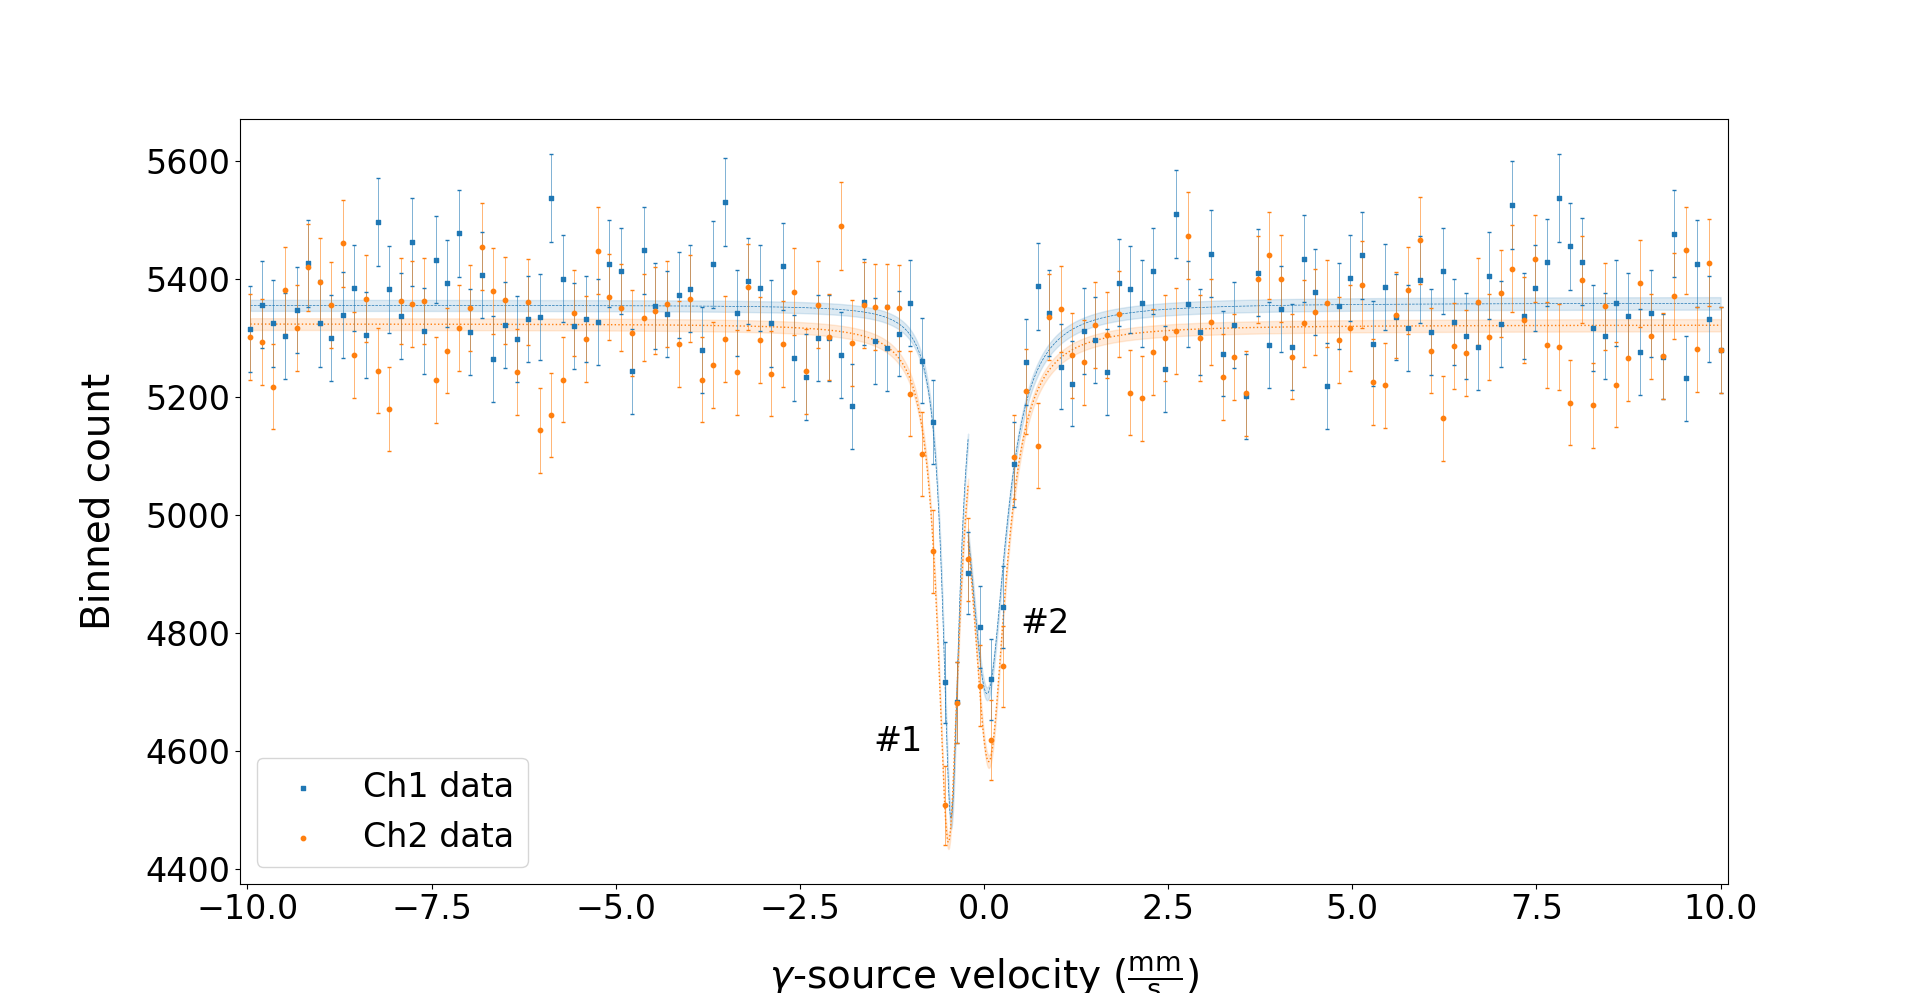
\includegraphics[width=1.0\textwidth]{./fig/Phosphate.png}
	\caption{Mössbauer spectrum of FePO$_4$}{}
\end{figure}

\begingroup
\renewcommand{\arraystretch}{1.3}
\begin{table}
	\begin{center}
	\caption{Mössbauer spectrum fit parameters for phosphate}
	\begin{tabular*}{0.9\textwidth}{@{\extracolsep{\fill}} c|ccccc}
  \toprule
	\hline
  Peak \# & $\Upphi_0$ & $A$ & $v_0$ & $\Gamma$ & Channel \\
	\hline
  \multirow{2}{*}{\#1} & $5355\pm9$ & $16\pm7.1$ & $-0.45\pm0.01$ & $0.275\pm0.080$ & Ch1 \\
                       & $5323\pm10$ & $28\pm7.4$ & $-0.48\pm0.02$ & $0.358\pm0.057$ & Ch2 \\
                       \hline
  \multirow{2}{*}{\#2} & $5359\pm11$ & $64\pm17.9$ & $0.04\pm0.03$ & $0.622\pm0.103$ & Ch1 \\
                       & $5322\pm10$ & $57\pm13.9$ & $0.06\pm0.02$ & $0.557\pm0.080$ & Ch2 \\
                       \hline
    \bottomrule
		\end{tabular*}
		\label{tab:phosphate}
	\end{center}

\end{table}
\endgroup

